% SC2000 — Chapter 3: Conditional Probability & Bayes
\chapter{Conditional Probability \& Bayes' Theorem}
\label{ch:conditional}

\begin{quote}
\emph{``Information changes belief.''} You tested positive for a rare disease---how worried should you be? An email contains the word ``lottery''---is it spam? Both are conditional probability questions: $P(\text{truth}\mid\text{evidence})$, not $P(\text{evidence}\mid\text{truth})$. Mixing the two is the most expensive mistake in applied statistics.
\end{quote}

\noindent\fbox{\parbox{\dimexpr\linewidth-2\fboxsep-2\fboxrule}{%
\textbf{From zero: we build on sample spaces (Ch.~2).} Conditional probability is just ``zoom into the part of $\Omega$ we now know occurred and renormalise.'' Bayes' rule flips the conditioning direction; independence means learning $B$ tells you nothing about $A$.}}
\vspace{0.4em}

\section*{Learning Outcomes}
After this chapter you will be able to:
\begin{enumerate}[label=(L\arabic*)]
    \item compute $P(A\mid B)$ from the definition and interpret it as renormalisation;
    \item apply the law of total probability to partition evidence;
    \item state and apply Bayes' theorem, including the odds form;
    \item recognise and test (pairwise/mutual) independence;
    \item diagnose base-rate fallacy and Simpson's paradox in real data.
\end{enumerate}

% ============================================================
\section{Conditional Probability}
\label{sec:conditional-def}

\begin{definition}[Conditional probability] For $P(B)>0$,
\[
P(A\mid B)=\frac{P(A\cap B)}{P(B)}.
\]
Read ``probability of $A$ given $B$''.
\end{definition}

\emph{Picture:} condition on $B$ = discard everything outside $B$, rescale what remains so $B$ has total mass $1$. Formally, $P(\cdot\mid B)$ itself satisfies Kolmogorov's axioms on the new sample space $B$.

\begin{figure}[h]
\centering
\begin{tikzpicture}[scale=0.75,every node/.style={font=\scriptsize}]
% Venn with conditioning
\draw[thick,rounded corners=4pt] (-3.3,-1.75) rectangle (3.3,1.75);
\node[font=\tiny] at (-2.75,1.5) {$\Omega$};
\draw[thick,fill=blue!12] (-1.2,0) ellipse (1.6 and 1.1);
\draw[thick,fill=orange!16] (0.85,0) ellipse (1.5 and 1.1);
\node at (-1.2,0) {$A$}; \node at (0.85,0) {$B$};
% highlight A cap B
\begin{scope}
\clip (-1.2,0) ellipse (1.6 and 1.1);
\fill[violet!28] (0.85,0) ellipse (1.5 and 1.1);
\end{scope}
\draw[thick,fill=violet!28,fill opacity=0.0] (0.85,0) ellipse (1.5 and 1.1);
\draw[thick] (-1.2,0) ellipse (1.6 and 1.1);
\node[font=\tiny,fill=white,inner sep=1pt,rounded corners=2pt] at (-0.05,0.05) {$A\cap B$};
\node[font=\tiny,align=center] at (0,-2.25) {$P(A\mid B)=\dfrac{P(A\cap B)}{P(B)}$ = share of $B$ covered by $A$};
% arrow to zoomed view
\draw[->,thick,violet!70!black] (3.75,0)--(4.55,0) node[midway,above,font=\tiny] {zoom into $B$};
\begin{scope}[xshift=6.3cm]
\draw[thick,fill=orange!16,rounded corners=4pt] (-1.5,-1.15) rectangle (1.5,1.15);
\node[font=\tiny] at (0,1.38) {New $\Omega'=B$ (rescaled to mass $1$)};
\begin{scope}
\clip (-1.5,-1.15) rectangle (1.5,1.15);
\fill[violet!28] (-0.15,0) ellipse (1.05 and 0.72);
\draw[thick] (-0.15,0) ellipse (1.05 and 0.72);
\end{scope}
\node[font=\tiny] at (-0.15,0) {$A\cap B$};
\node[font=\tiny,align=center] at (0,-1.65) {$P(A\mid B)$ is its share};
\end{scope}
\end{tikzpicture}
\caption{Conditioning on $B$ zooms into $B$ and renormalises. $P(A\mid B)$ is the fraction of $B$'s mass that also lies in $A$.}
\label{fig:conditional}
\end{figure}

\begin{example}[Two dice, given at least one $6$] $P(\text{sum }7\mid\text{at least one }6)=|A\cap B|/|B|=1/11$ (only $(1,6)$ qualifies among $11$ outcomes with a $6$). Unconditionally $P(\text{sum }7)=1/6$; the information ``a $6$ appeared'' changes the probability.
\end{example}

Properties: $P(\cdot\mid B)$ is a probability measure; chain rule $P(A\cap B)=P(A\mid B)P(B)$; $P(A^c\mid B)=1-P(A\mid B)$.

% ============================================================
\section{Law of Total Probability}
\label{sec:total-prob}
If $B_1,\dots,B_k$ partition $\Omega$ (disjoint, union $=\Omega$, each $P(B_i)>0$),
\[
P(A)=\sum_{i=1}^k P(A\mid B_i)\,P(B_i).
\]
\emph{Intuition:} slice $\Omega$ into cases $B_i$, compute $P(A)$ within each slice, weight by slice size. This is how we handle ``$A$ can happen via several mutually exclusive pathways.''

\begin{example}[Email spam via law of total probability] $60\%$ of mail is spam ($S$), $40\%$ ham ($H$). Word ``lottery'' appears in $30\%$ of spam, $2\%$ of ham. Then
\[
P(\text{``lottery''})=0.30\cdot0.60+0.02\cdot0.40=0.188.
\]
\end{example}

% ============================================================
\section{Bayes' Theorem}
\label{sec:bayes}

\begin{theorem}[Bayes' theorem] For $P(B)>0$,
\[
P(B_j\mid A)=\frac{P(A\mid B_j)\,P(B_j)}{\sum_i P(A\mid B_i)\,P(B_i)}=\frac{P(A\mid B_j)\,P(B_j)}{P(A)}.
\]
\end{theorem}
It \emph{inverts} conditioning: from $P(\text{evidence}\mid\text{hypothesis})$ and prior $P(\text{hypothesis})$ to posterior $P(\text{hypothesis}\mid\text{evidence})$.

\begin{corollary}[Odds form] $\displaystyle\frac{P(B\mid A)}{P(B^c\mid A)}=\frac{P(A\mid B)}{P(A\mid B^c)}\cdot\frac{P(B)}{P(B^c)}$. Posterior odds = likelihood ratio $\times$ prior odds.
\end{corollary}

\begin{figure}[h]
\centering
\begin{tikzpicture}[scale=0.74,every node/.style={font=\scriptsize}]
% Bayes tree: prior -> likelihood -> posterior
\node[draw,rounded corners=3pt,fill=blue!12,inner sep=4pt] (prior) at (0,0) {\textbf{Prior} $P(S)=0.6$};
\node[draw,rounded corners=3pt,fill=orange!14,inner sep=4pt] (like) at (4.5,0) {\textbf{Likelihood} $P(W\mid S)=0.30$};
\node[draw,rounded corners=3pt,fill=green!14,inner sep=4pt] (post) at (9.2,0) {\textbf{Posterior} $P(S\mid W)=\dfrac{0.18}{0.188}\approx0.957$};
\draw[->,thick,blue!60!black] (prior)--(like) node[midway,above,font=\tiny] {observe $W$};
\draw[->,thick,orange!70!black] (like)--(post) node[midway,above,font=\tiny] {Bayes};
% second row: medical test tree
\begin{scope}[yshift=-2.6cm]
\node[font=\footnotesize\bfseries] at (0,1.05) {Medical test tree (base-rate demo):};
% root
\node[circle,draw,fill=blue!10,inner sep=2pt] (r) at (0,0) {};
\node[font=\tiny,above=1pt of r] {Pop.};
% disease branch
\node[draw,fill=red!12,rounded corners=2pt,inner sep=2pt] (d) at (-2.8,-1.0) {$D$ $1\%$};
\node[draw,fill=green!10,rounded corners=2pt,inner sep=2pt] (nd) at (2.0,-1.0) {$\neg D$ $99\%$};
\draw[thick] (r)--(d) node[midway,left,font=\tiny] {$0.01$};
\draw[thick] (r)--(nd) node[midway,right,font=\tiny] {$0.99$};
% test results
\node[draw,fill=red!18,rounded corners=2pt,inner sep=2pt] (tp) at (-4.2,-2.15) {$+$ $90\%$};
\node[draw,fill=red!8,rounded corners=2pt,inner sep=2pt] (fn) at (-1.2,-2.15) {$-$ $10\%$};
\node[draw,fill=orange!14,rounded corners=2pt,inner sep=2pt] (fp) at (0.7,-2.15) {$+$ $9\%$};
\node[draw,fill=green!12,rounded corners=2pt,inner sep=2pt] (tn) at (3.0,-2.15) {$-$ $91\%$};
\draw[thick] (d)--(tp) node[midway,left,font=\tiny] {$0.9$};
\draw[thick] (d)--(fn) node[midway,right,font=\tiny] {$0.1$};
\draw[thick] (nd)--(fp) node[midway,left,font=\tiny] {$0.09$};
\draw[thick] (nd)--(tn) node[midway,right,font=\tiny] {$0.91$};
\node[font=\tiny,align=center,fill=yellow!14,rounded corners=2pt,inner sep=2pt] at (0,-3.1) {Posterior $P(D\mid+)=\dfrac{0.01\cdot0.9}{0.01\cdot0.9+0.99\cdot0.09}\approx9.2\%$ --- low despite $90\%$ sensitivity!};
\end{scope}
\end{tikzpicture}
\caption{Top: Bayes as prior $\to$ likelihood $\to$ posterior. Bottom: medical test tree showing the base-rate fallacy.}
\label{fig:bayes-tree}
\end{figure}

\begin{example}[Rare disease, base-rate fallacy] Disease prevalence $1\%$, test sensitivity $90\%$, false-positive rate $9\%$. Then
\[
P(D\mid+)=\frac{0.9\cdot0.01}{0.9\cdot0.01+0.09\cdot0.99}\approx0.092.
\]
Even after testing positive, only $\approx9\%$ chance of disease! The error is confusing $P(+\mid D)=0.9$ with $P(D\mid+)$. Always account for the base rate $P(D)$.
\end{example}

% ============================================================
\section{Independence}
\label{sec:independence}

\begin{definition}[Independence] Events $A,B$ are \emph{independent} if $P(A\cap B)=P(A)P(B)$, equivalently $P(A\mid B)=P(A)$ when $P(B)>0$. A family is \emph{mutually independent} if every finite subcollection factorises; \emph{pairwise independent} is weaker.
\end{definition}

\emph{Computing relevance:} independent failures multiply: $P(\text{all $n$ replicas fail})=p^n$ if each fails with prob.\ $p$ independently. Hash collisions, randomised algorithms, and naive Bayes classifiers all assume (or approximate) independence.

\begin{example}[Pairwise but not mutual] Two fair coin tosses: $A=\{\text{first }H\}$, $B=\{\text{second }H\}$, $C=\{\text{tosses agree}\}$. Each pair independent ($1/4=1/2\cdot1/2$), but $P(A\cap B\cap C)=1/4\ne1/8$. Pairwise $\not\Rightarrow$ mutual.
\end{example}

% ============================================================
\section{Simpson's Paradox (Preview)}
Aggregated data can reverse trends seen in every subgroup. E.g., treatment $A$ beats $B$ in both men and women separately, yet $B$ beats $A$ overall---because group sizes differ (a conditioning effect). Always condition on relevant covariates; see Ch.~8 for regression's resolution.

\begin{example}[Simpson's numbers] Department X: treatment $A$ cures $80/100$ ($80\%$) vs.\ $B$ $30/40$ ($75\%$); department Y: $A$ $20/40$ ($50\%$) vs.\ $B$ $10/100$ ($10\%$). In each department $A$ wins, but overall $A$ is $100/140\approx71\%$ while $B$ is $40/140\approx29\%$ here $A$ still wins---to flip it, swap group sizes: if $A$ treated mostly hard cases, aggregate can reverse. Real Berkeley admissions (1973) showed exactly this structure.
\end{example}

% ============================================================
\section{Computing Bayes in Code}
\label{sec:code-bayes}

\begin{lstlisting}[language=Python]
# Bayes: spam filter and medical test
def bayes_posterior(prior, likelihood_pos, false_pos):
    """P(D|+) from prior P(D), P(+|D), P(+|~D)."""
    num = likelihood_pos * prior
    den = likelihood_pos * prior + false_pos * (1 - prior)
    return num / den

print(f"P(spam|'lottery') = {bayes_posterior(0.6, 0.30, 0.02):.3f}")  # 0.957
print(f"P(disease|+) = {bayes_posterior(0.01, 0.90, 0.09):.3f}")     # 0.092

# Chain rule demo: P(A,B,C) = P(A)*P(B|A)*P(C|A,B)
# Naive Bayes assumes P(features|class) factorises
\end{lstlisting}

% ============================================================
\section{Chapter Notes}
Bayes' theorem appears in Bayes (1763, posthumous) and Laplace (1774). The base-rate fallacy is Kahneman--Tversky's classic; Gerd Gigerenzer advocates natural frequencies (``9 of 98 positives are diseased'') to make Bayes intuitive. Naive Bayes classifiers (Ch.~8) exploit conditional independence for text classification despite the ``naive'' assumption.

% ============================================================
\section{Exercises}
\label{sec:ch03-exercises}
\begin{enumerate}[label=E3.\arabic*, leftmargin=*, itemsep=0.8em]
\item \textbf{Conditional drill.} Two fair dice are rolled. Compute (a) $P(\text{sum }8\mid\text{at least one }4)$, (b) $P(\text{doubles}\mid\text{sum }\le6)$. Draw the relevant subgrids.
\item \textbf{Law of total probability.} A factory has machines $M_1,M_2,M_3$ producing $30\%,50\%,20\%$ of chips with defect rates $2\%,1\%,5\%$. A random chip is defective---what is $P(M_2\mid\text{defective})$ via Bayes?
\item \textbf{Base-rate fallacy.} An intrusion detector has $99\%$ detection rate and $1\%$ false-alarm rate. Attacks occur in $0.1\%$ of connections. Compute $P(\text{attack}\mid\text{alarm})$. How many alarms are false? Propose how to improve precision.
\item \textbf{Independence.} (a) Prove if $A,B$ independent then $A^c,B$ independent. (b) Construct three events pairwise independent but not mutually independent (verify all conditions numerically).
\item \textbf{Odds form.} Derive the odds form of Bayes. A spam filter has prior odds $3{:}2$ for spam and likelihood ratio $15$ for word ``prize''. Compute posterior odds and convert to probability.
\end{enumerate}
% End of Chapter 3
